\section{Typische Anwendungen des BLDC-Motors}

Viele Funktionen, die früher zum Aufgabengebiet der bürstenbehafteten Motoren gehörten werden mittlerweile von bürstenlosen Gleichstrommotoren erfüllt. Jedoch hindern Kosten und hoher Steuerungsaufwand den Motorentyp daran, seinen Vorgänger vollständig abzulösen.

Trotzdem dominieren BLDC-Motoren heutzutage besonders in Anwendungsgebieten, bei denen ein niederer Wartungsaufwand, hohe Motordrehzahlen, hohe Zuverlässigkeit und hohe Effizienz zu den Anforderungen gehören. Es folgt ein kurzer Überblick über die typischen Anwendungsgebiete des BLDC-MotorS.  Danach wird ein detailliertes Anwendungsbeispiel ausgeführt.

\subsection{Überblick}

\paragraph{Fortbewegungsmittel:} Mittlerweile finden sich bürstenlose Gleichstrommotoren in radgetriebenen Fahrzeugen jeglicher Größe. Vom elektrisch untertützten Fahrrad \parencite[S. 6]{Xia2012} bis zum elektrisch angetriebenen Lastkraftwagen werden BLDC-Motoren in nahezu jedem Segment der Fortbewegungs- und Transportmittel eingesetzt. Eine mögliche Anwendung ist die Ausführung als Radnabenmotor, welche in Abbildung \ref{fig:Radnabenmotor} dargestellt ist.
\begin{figure}[h]
  \centering
  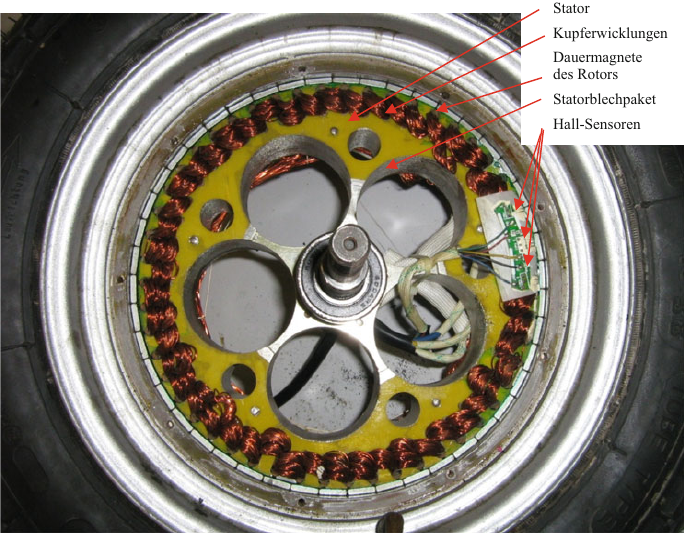
\includegraphics[width=10cm]{Radnabenmotor}
  \caption[Radnabenmotor]{Radnabenmotor (Quelle: \parencite[S. 132]{Babiel2014})}
  \label{fig:Radnabenmotor}
\end{figure}
Hier kann besonders von der hohen Effizienz des Motors profitiert werden, da durch diese Eigenschaft höhere Batterielaufzeiten erzielt werden können \parencite[S. 4]{Xia2012}. Da Elektromotoren hier nicht nur für den Antrieb des Fahrzeugs, sondern auch für Fensterheber, Airbags, Scheibenwischer, Schließmechanismen und vieles mehr genutzt werden können werden in einem durchschnittlichen Personenkraftwagen Dutzende, wenn nicht gar hunderte Elektromotoren verbaut \parencite[S. 4]{Xia2012}.

\paragraph{Batteriebetriebenes Werkzeug:} Bei Anwendungen im handwerklichen Alltag werden bürstenlose Motoren besonders in Sägen, Bohrmaschinen, Laubgebläsen, Rasentrimmern und vielem mehr verwendet. Von vielen der genannten Maschinen finden sich auf der Baustelle kabelgebundene Versionen, die jedoch einige Nachteile mit sich bringen. Nennenswert wären zum Beispiel Kabelmanagement und die damit verbundene Not einer Stromversorgung, die bei einem Neubau oftmals erst durch einen kommunalen Stromverteiler gelegt werden musS.  Durch die Verwendung von BLDC-Motoren verringert sich die Leistungsanforderung des Geräts drastisch, sodass nun Geräte mit Batterieversorgung entwickelt und gebaut werden können, die an einem zentralen Punkt der Baustelle nachgeladen werden können, ohne ein kompliziertes Netzwerk aus Stromverteilern und Verlängerungskabeln aufbauen zu müssen. Ein weiterer Vorteil liegt in der Gewichtsersparnis der Maschinen, denn durch die höhere Leistungsdichte eines BLDC-Motors kann ein kleinerer Motor bei selber Leistung verwendet werden. In der untenstehenden Abbildung \ref{fig:Vergleich} wird zudem der Größenunterschied gut sichtbar. Das bürstenlose Modell (rechts) kann weitaus kompakter gebaut werden und verfügt trotzdem über 50\% mehr Drehmoment (\SI{60}{\newton\meter})als das bürstenbehaftete Modell (\SI{40}{\newton\meter}). Auf das Modell DDF481 im Bild rechts, welches mit einem bürstenlosen Motor ausgestattet ist soll im nächsten Abschnitt noch detaillierter eingegangen werden.

\begin{figure}[H]
  \centering
  %------------------------------
  \begin{minipage}{.49\textwidth}
    \centering
    \includegraphics[height=5cm]{Makita_Bürstenbehaftet}
  \end{minipage}\hfill%
  \begin{minipage}{.49\textwidth}
    \centering
    \includegraphics[height=5cm]{Makita_Bürstenlos}
  \end{minipage}
  \caption[Vergleich Akkubohrschrauber]{Vergleich zweier Akku-Bohrschrauber der Firma Makita. Links: Modell DDF451, bürstenbehafteter Antrieb, Gehäuselänge: \SI{238}{\milli\meter}. Rechts: Modell DDF481, bürstenloser Antrieb, Gehäuselänge: \SI{205}{\milli\meter}. (Quelle: Fa. Makita)}
  \label{fig:Vergleich}
\end{figure}

\paragraph{Haushaltsgeräte:} In der letzten Zeit wurden weltweit jährlich etwa 30\% mehr Elektromotoren in Haushaltsgeräten verbaut. Mit dem steigenden Lebensstandard der Menschen und dem wachsenden Umweltbewusstsein sind bürstenlose Gleichstrommotoren immer mehr das Mittel der Wahl im alltäglichen Gebrauch; so auch im Haushalt \parencite[S. 6]{Xia2012}. Lüfter sind ein Anwendungsgebiet, in dem man mittlerweile ausschließlich bürstenlose Gleichstrommotoren vorfindet. Auch hier wird insbesondere von der Leistungsersparnis profitiert. Ein weiterer Vorteil im Segment der Lüfter und Ventilatoren (auch Haartrockner, Heizlüfter etc.) besteht in der Tatsache, dass die Lautstärke des Geräts abnimmt, da keine mechanische Reibung bei der Kommutation entsteht.

\paragraph{Modellfluggeräte:} Das Wachstum der Popularität von ferngesteuerten Modellfluggeräten --- insbesondere Drohnen und Quadrokoptern --- wurde maßgeblich durch die Entwicklung des BLDC-Motors angestoßen. Im Bereich der Fluggeräte wurden seither stets kleine Verbrennungsmotoren eingesetzt. In einigen Staaten wurden Verbrennungsmotoren für diese Anwendung mittlerweile verboten, da die Lärmverschmutzung als zu hoch eingestuft wurde. Auch hier zeigen sich die Vorteile des bürstenlosen GleichstrommotorS.  Zusätzlich sorgt die Einsetzung dieses neuen Motortyps für eine höhere Reichweite, da eine kleineres Verhältnis von Gewicht und Leistung vorliegt.

\paragraph{Industrielle Anwendungen:} Im industriellen Umfeld spielt der BLDC-Motor insbesondere in der Produktion, sowie der industriellen Automatisierung eine große Rolle. Bürstenlose Motoren sind für diese Funktionen besonders gut geeignet, da sie sich durch eine hohe Leistungsdichte, hohe Effizienz, große Drehzahlbereiche und niederen Wartungsaufwand auszeichnen \parencite[S. 8]{Xia2012}. In der Produktion werden sie vor allem für Bewegungsregelung, Positionierung und Aktorik verwendet.

\subparagraph{Bewegungsregelung:} Bürstenlose Gleichstrommotoren werden häufig als Treiber für Pumpen, Lüfter und Spindeln, beispielsweise in CNC-Fräsen eingesetzt. Aufgrund ihrer Konstruktion verfügen BLDC-Motoren über gute thermische Eigenschaften und eine hohe Effizienz. Hinzu kommt die niederere Massenträgheit im Vergleich mit dem bürstenbehafteten Motor. All dies sind Eigenschaften, die den BLDC-Motor für dieses Einsatzgebiet prädestinieren.

\subparagraph{Positionierungs- und Aktuatoriksysteme:} BLDC-Motoren werden als Aktorik- und Positionierungssysteme in der Industrie eingesetzt \parencite[S. 159]{Gopal2002}. In diesem Anwendungsgebiet trifft man besonders bürstenlose Servo- oder Schrittmotoren an, beispielsweise in Industrierobotern. Darüber hinaus können bürstenlose Gleichstrommotoren auch dazu verwendet werden, Linearaktuatoren anzutreiben \parencite[S. 91]{Zhang2013} (S.  dazu auch Abbildung \ref{fig:Linearantrieb}).

\begin{figure}[H]
  \begin{minipage}{.47\textwidth}
    \centering
    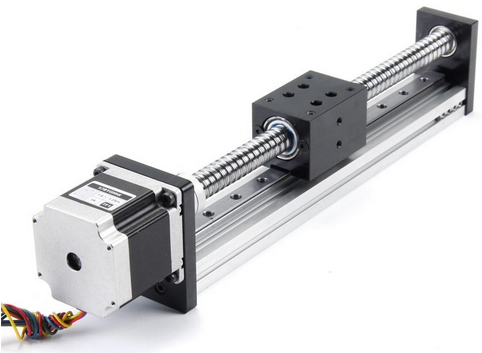
\includegraphics[height=6cm]{Linearantrieb}
    \caption[Linearantrieb mit BLDC-Motor]{Linearantrieb mit BLDC-Motor (Quelle: Fa. Banggood)}
    \label{fig:Linearantrieb}
  \end{minipage}\hfill%
  \begin{minipage}{.47\textwidth}
    \centering
    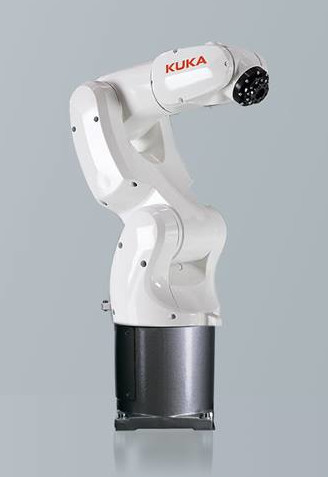
\includegraphics[height=6cm]{Industrieroboter}
    \caption[Industrieroboter KR 3 Agilus]{Industrieroboter KR 3 Agilus (Quelle: Fa. Kuka)}
    \label{fig:Industrieroboter}
  \end{minipage}
\end{figure}

Im nächsten Abschnitt wird der Einsatz von bürstenlosen Gleichstrommotoren exemplarisch anhand eines Akkubohrschraubers beschrieben.

\subsection{Ausführliches Anwendungsbeispiel}

\glqq{}Die Marke Makita steht weltweit für professionelle und qualitativ hochwertige Akku-, Elektro- und Benzin-Werkzeuge. Gerade im Akku-Bereich setzt Makita immer wieder neue Maßstäbe. Auch in Deutschland ist Makita seit 1977 vertreten und verfügt über ein riesiges Produktsortiment und das passende Zubehör\grqq{} (\url{www.makita.de}). Im Produktportfolio findet sich unter anderem der Akkubohrschrauber DDF481 --- Makitas stärkstes Gerät in diesem Segment. Der DDF481 wird von einem bürstenlosen Gleichstrommotor angetrieben. Mithilfe dieses Antriebs gelang es Makita, die Gehäuselänge trotz einer höheren Leistung maßgeblich zu verkürzen. Somit benötigt der DDF481 weniger Stauraum im Koffer eines Handwerkers oder in der Werkstatt eines Privathaushalts. Zudem kann in engeren Spalten gebohrt und geschraubt werden.

Das Gerät wird von einem bürstenlosen Gleichstrommotor in Innenläuferausführung angetrieben, der Drehmomente von bis zu \SI{110}{\newton\meter} erlaubt. Der Motor wird von Makita selbst hergestellt.

\begin{figure}[h]
  \centering
  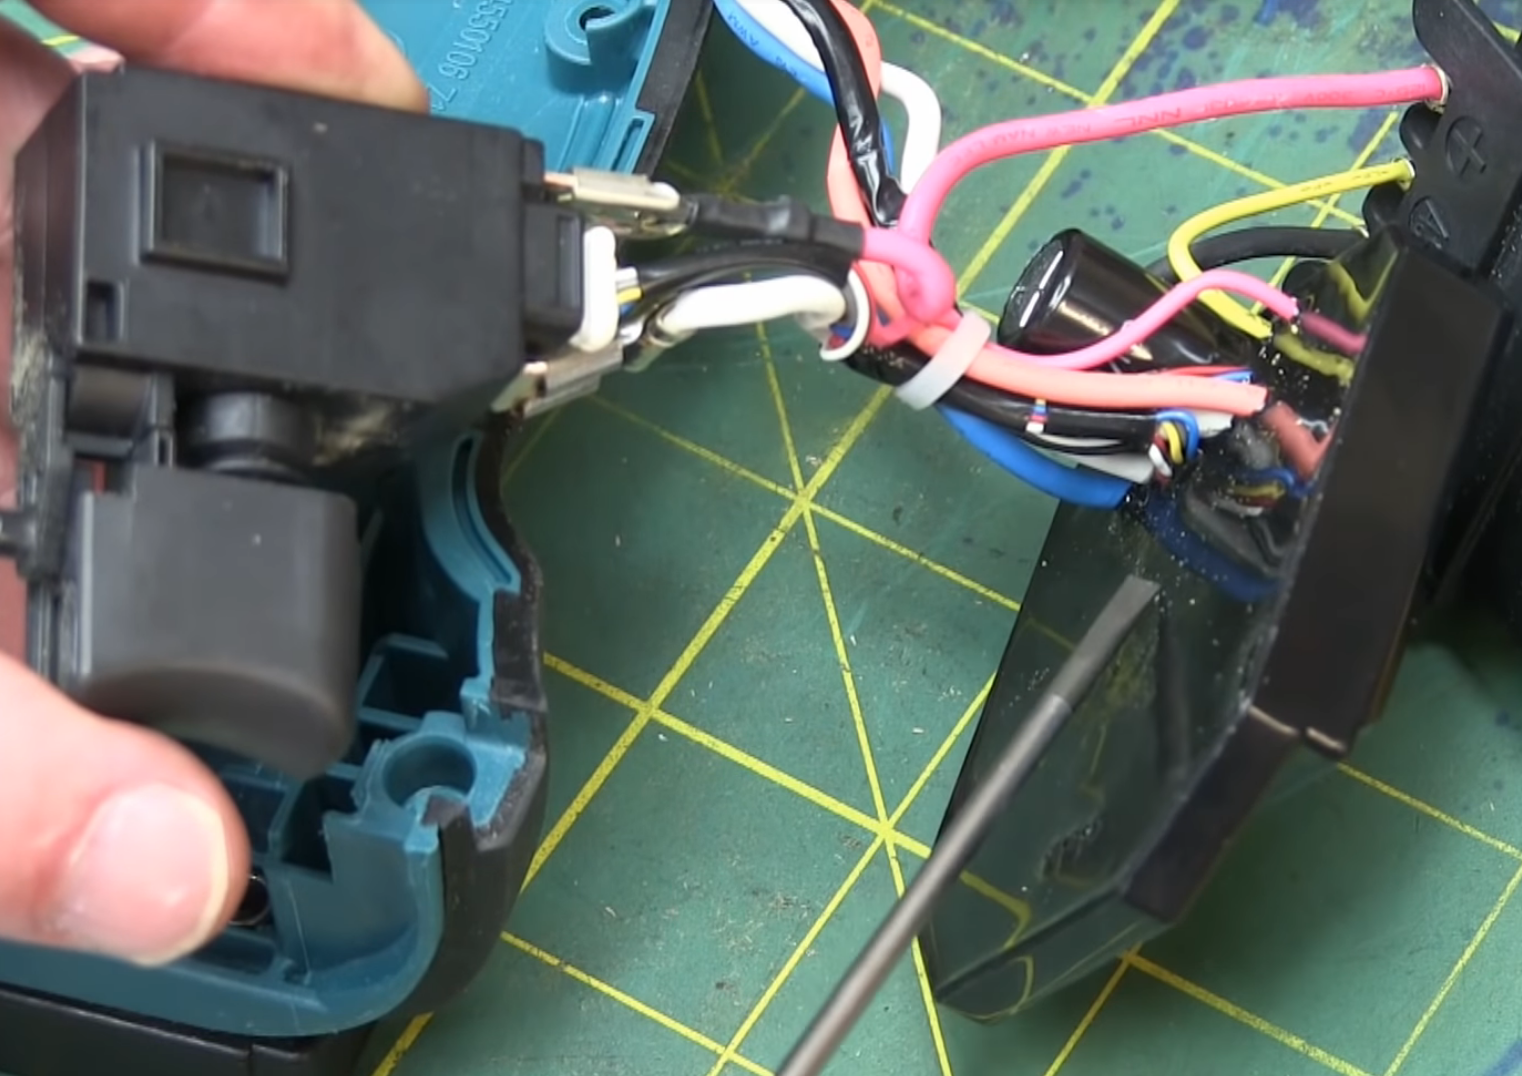
\includegraphics[width=.5\textwidth]{Makita_DDF481_Steuerung}
  \caption{Steuerung des DDF481 (Quelle: YouTube-Kanal \glqq{}ave\grqq{})}
  \label{fig:Steuerung}
\end{figure}

In Abbildung~\ref{fig:Steuerung} ist das Steuerungsmodul des Bohrschraubers zu sehen. Das Modul selbst ist in Epoxidharz vergossen, um die Elektronik vor Schmutz und Feuchtigkeit zu schützen. Das Elektronikmodul misst den vom Schalter (links im Bild) abgegriffenen Widerstandswert und berechnet daraus die zu liefernde Motorendrehzahl. Diese mit Hilfe der integrierten Sensorik des Motors vom Elektronikmodul geregelt.

\begin{figure}[h]
  \begin{minipage}{.48\textwidth}
    \centering
    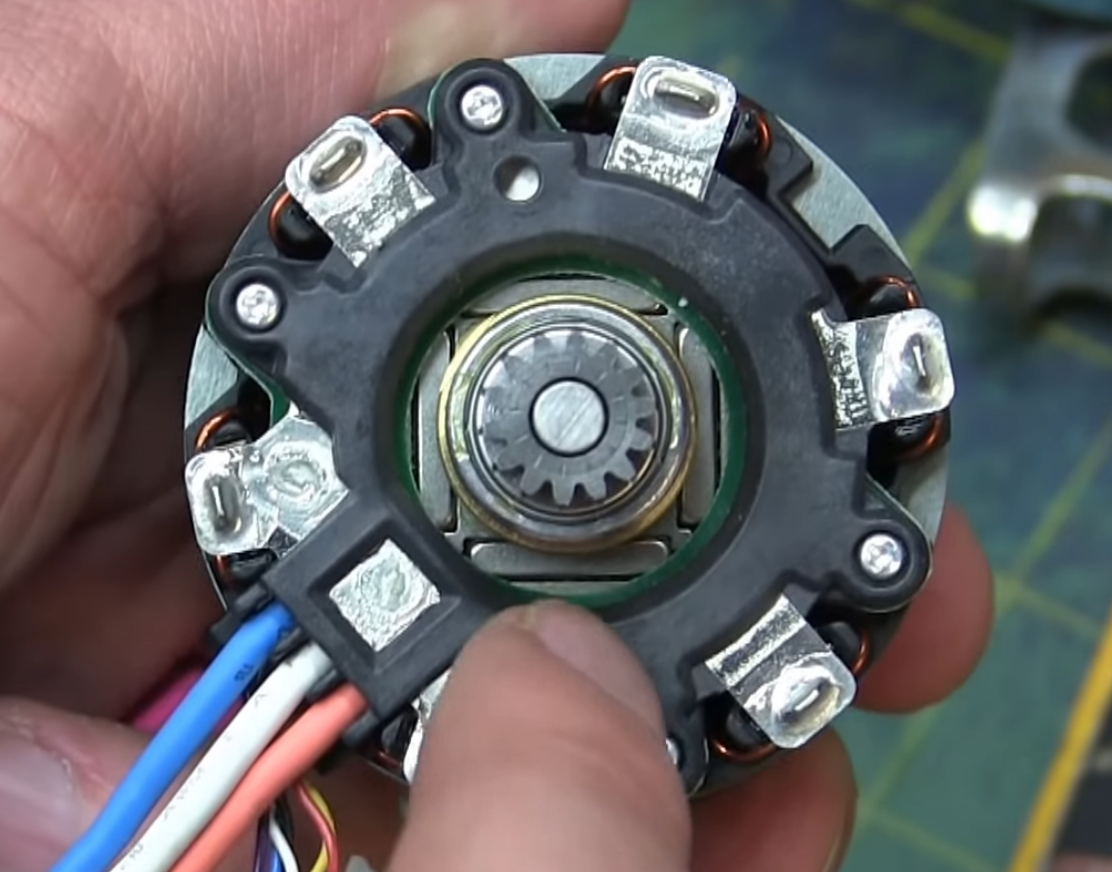
\includegraphics[height=5cm]{Makita_DDF481_Feld}
    \caption{Vorderansicht des Motors (Quelle: YouTube-Kanal \glqq{}ave\grqq{})}
    \label{fig:Feld}
  \end{minipage}\hfill%
  \begin{minipage}{.48\textwidth}
    \centering
    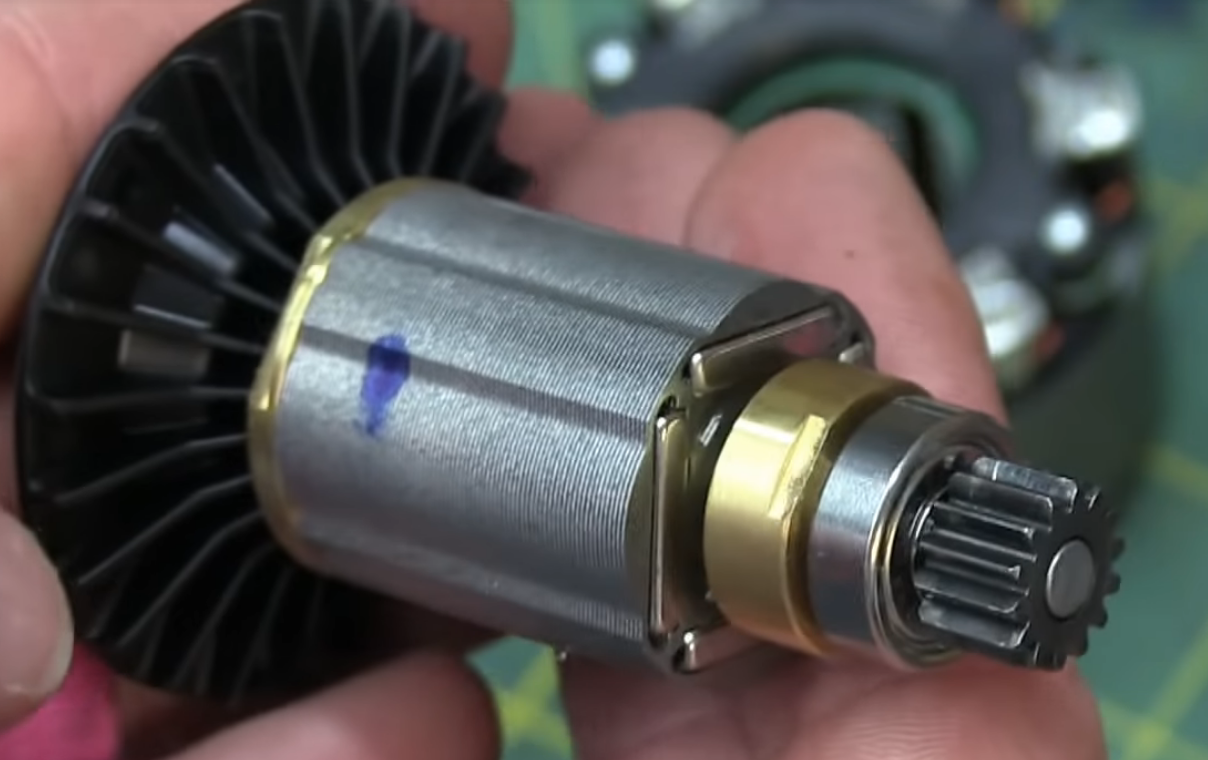
\includegraphics[height=5cm]{Makita_DDF481_Anker}
    \caption{Anker des Motors (Quelle: YouTube-Kanal \glqq{}ave\grqq{})}
    \label{fig:Anker}
  \end{minipage}
\end{figure}

Der Motor verfügt über drei Polpaare (siehe Abbildung~\ref{fig:Feld}), welche nacheinander beschaltet werden. In Abbildung~\ref{fig:Anker} ist der Permanentmagnetkern des Motors zu sehen. Hier wird deutlich, dass es dieser Motor in Innenläuferausführung aufgebaut ist. Die gefächerte Struktur des hinteren Ankerbereichs --- zu sehen in Abbildung~\ref{fig:Anker} --- sorgt für zusätzlich kühlende Luftströmungen während des Betriebs.

%%% Local Variables:
%%% mode: latex
%%% TeX-master: "BLDC"
%%% End:
